% 导言区
\documentclass{ctexart}

\usepackage{ctex}
\usepackage{graphicx}
\graphicspath{{figures/}}

% 正文区(文稿区)
\begin{document}

	% 图像浮动体环境,可将图片放入此环境中
	\begin{figure}[htbp]
		% 可以采用centering 让环境中的内容居中排版
		\centering
		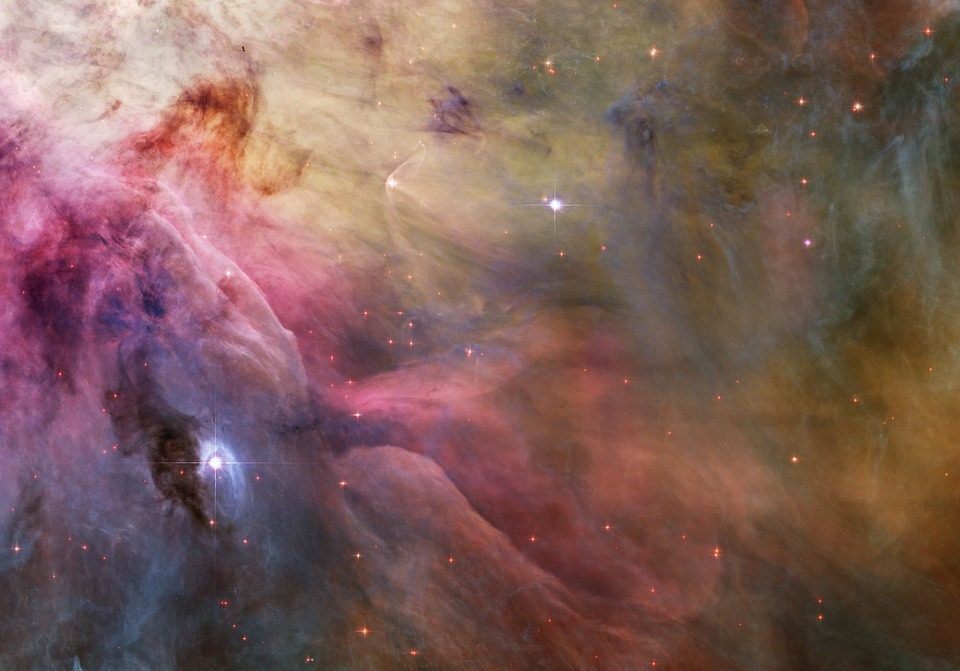
\includegraphics[scale=0.3]{1.jpg}
		% \caption命令设置图片标题
		\caption{text}
	\end{figure}

	在LaTex中也可以这样使用表\ref{tab-score}所示的表格
	% 表格浮动体环境,可将表格放入此环境中
	\begin{table}
		\centering
		\caption{考试成绩单}\label{tab-score}
		\begin{tabular}{|l|c|c|c|r|}
			\hline
			姓名 & 语文 & 数学 & 操作系统 & 数据结构 \\
			\hline
			yuluo & 100 & 100 & 100 & 100 \\
			\hline
			huakai & 100 & 100 & 100 & 100 \\
			\hline
		\end{tabular}
	\end{table}

	% 使用tabular环境生成表格
	% 有一个必选参数,指定表格的内容对齐格式
	% l 左对齐 c 居中 r 右对齐 用\\结尾
	%  可以使用\\hline产生横线
	% 可以使用两个\\hline和两个 || 产生双竖线 
	\begin{tabular}{|l|c|c|c|r|}
	\hline
		姓名 & 语文 & 数学 & 操作系统 & 数据结构 \\
	\hline
		yuluo & 100 & 100 & 100 & 100 \\
	\hline
		huakai & 100 & 100 & 100 & 100 \\
	\hline
	\end{tabular}

	% 可以用p参数指定列格式的宽度,内容超过宽度时自动换行
	\begin{tabular}{|l|c|c|c|p{1.5cm}|}
	\hline
		姓名 & 语文 & 数学 & 操作系统 & 数据结构 \\
	\hline
		yuluo & 100 & 100 & 100 & 100 \\
	\hline
		huakai & 100 & 100 & 100 & 100 \\
	\hline
	\end{tabular}

\end{document}